\chapter{Testing}
È un'attività di verifica che permette di \textbf{controllare} che il software si comporti come lo sviluppatore e il cliente si aspettano. Coinvolge sia elementi \textbf{dinamici} che \textbf{statici}, perché verifica tutti gli \textbf{artefatti}.
\begin{itemize}
    \item  \textbf{\textcolor{brown}{Assicurazione di Qualità QA}}, che permette di progettare il software in modo che a partire dal progetto allo sviluppo, ci siano pochi errori.
    \item \textbf{\textcolor{brown}{Controllo della Qualità QC}}, una verifica finale che controlla che il codice sia esente da errori o ne abbia pochi.
\end{itemize}

\begin{boxDef}
\textbf{\textcolor{brown}{TESTING:}} è un esame \textbf{sistematico} e \textbf{metodico} di un prodotto che sfrutta una varietà di tecnologie e deve mostrare che soddisfa lo scopo richiesto. Si esegue il software in dei casi di test in un ambiente simile a quello di \textbf{produzione}, che spesso non è la stessa macchina dello sviluppo. \\
Posso far emergere l'errore tramite:
\begin{itemize}
    \item \textbf{Ispezioni}, in cui dei tester verificano a mano che il codice sia scritto in modo corretto.
    \item \textbf{Metodi formali}, come tecniche matematiche per verificare che sia corretto.
    \item Librerie di \textbf{\textcolor{blue}{analisi statica}} per evidenziare possibili errori.
\end{itemize}
\textbf{\textcolor{brown}{Unit Testing:}} il test di granularità più piccola che valuta i componenti a livello individuale, eseguiti dai tester e partecipa anche l'u tente con le beta.
\end{boxDef}

\section{Software Development Life Cycle (SDLC)}
Si comincia dal raccogliere i requisiti, prosegue con il design e termina con l'implementazione, in tutte va testato:
\begin{enumerate}
    \item \textbf{\textcolor{brown}{Test Statico:}} senza dover eseguire il codice.
    \item \textbf{\textcolor{brown}{Test Dinamico:}} esecuzione del codice e verifica del comportamento.
\end{enumerate}
Vengono testati i requisiti \textbf{\textcolor{blue}{funzionali}} e \textbf{\textcolor{blue}{non funzionali}}, rispettivamente basati sulle specifiche e in che modo le realizza.

\begin{itemize}
    \item \textbf{\textcolor{brown}{Test funzionali:}} controlla \textbf{completezza}, \textbf{correttezza} e \textbf{appropriatezza}, a partire dall'unità fino al quadro generale, normalmente \textbf{black box}.
    \item \textbf{\textcolor{brown}{Test non funzionali:}} focalizzato sulle qualità e gli attributi comportamentali come \textbf{usabilità}, \textbf{performance}, \textbf{efficienza} e \textbf{sicurezza}, sia \textbf{black} che \textbf{white box}.
    \begin{itemize}
        \item L'obiettivo è verificare la presenza di \textbf{problemi} di performance, valutando velocità, capacità, stabilità, scalabilità.
        \item Testing di \textbf{carico} e \textbf{stress} test per valutarlo sotto stress.
        \item Test di \textbf{usabilità} per valutare quanto tempo ci mette l'utente ad utilizzarlo.
        \item Test di \textbf{sicurezza} per valutare la protezione dei dati; test di portabilità per vedere quanto è portabile in altri ambienti di utilizzo.
        \item Test di \textbf{conformità} se è conforme agli standard; test di configurazione per vedere se funziona più configurazioni; test di UI se è consistente.
    \end{itemize}
\end{itemize}

Ci sono vari \textbf{livelli} e \textbf{fasi} di sviluppo del software che sono spesso correlate ad appositi test:
\begin{itemize}
    \item \textbf{\textcolor{brown}{Component unit testing:}} valutiamo la singola classe indipendente per valutare se soddisfa i requisiti funzionali, non funzionali per ridurre i rischi.
    \begin{itemize}
        \item Per ognuno bisogna individuare le basi del test, gli obiettivi dello stesso, i difetti tipici che possono verificarsi, l'approccio e le responsabilità.
    \end{itemize}
    \item \textbf{\textcolor{brown}{Integration testing:}} dopo aver unito insieme le unità testiamo le interfacce tra componenti e le loro interazioni.
    \begin{itemize}
        \item L'obiettivo è testare i sottosistemi e i database, API, microservizi per eliminare difetti di sequenza, comunicazione, codifica dei dati o errori.
        \item A livello di sistema valuta le interazioni tra sistemi, pacchetti o servizi anche esterni. Spesso coinvolge tester, partner per il testing.
    \end{itemize}
    \item \textbf{\textcolor{brown}{System testing:}} verifica l'intero sistema integrato e che sia corretta l'architettura sottostante individuando le stesse cose degli altri test.
    \item \textbf{\textcolor{brown}{User Acceptance testing:}} verifica che il sistema abbia raggiunto tutti i requisiti richiesti dall'utente per cui richiede la collaborazione dello stesso.
    \begin{itemize}
        \item Tra le forme di test di accettazione si ha UAT per l'utente, OAT di tipo operazionale, AT contrattuale e regolatorio, alpha e beta testing.
    \end{itemize}
\end{itemize}

\begin{figure}[!htb]
    \centering
    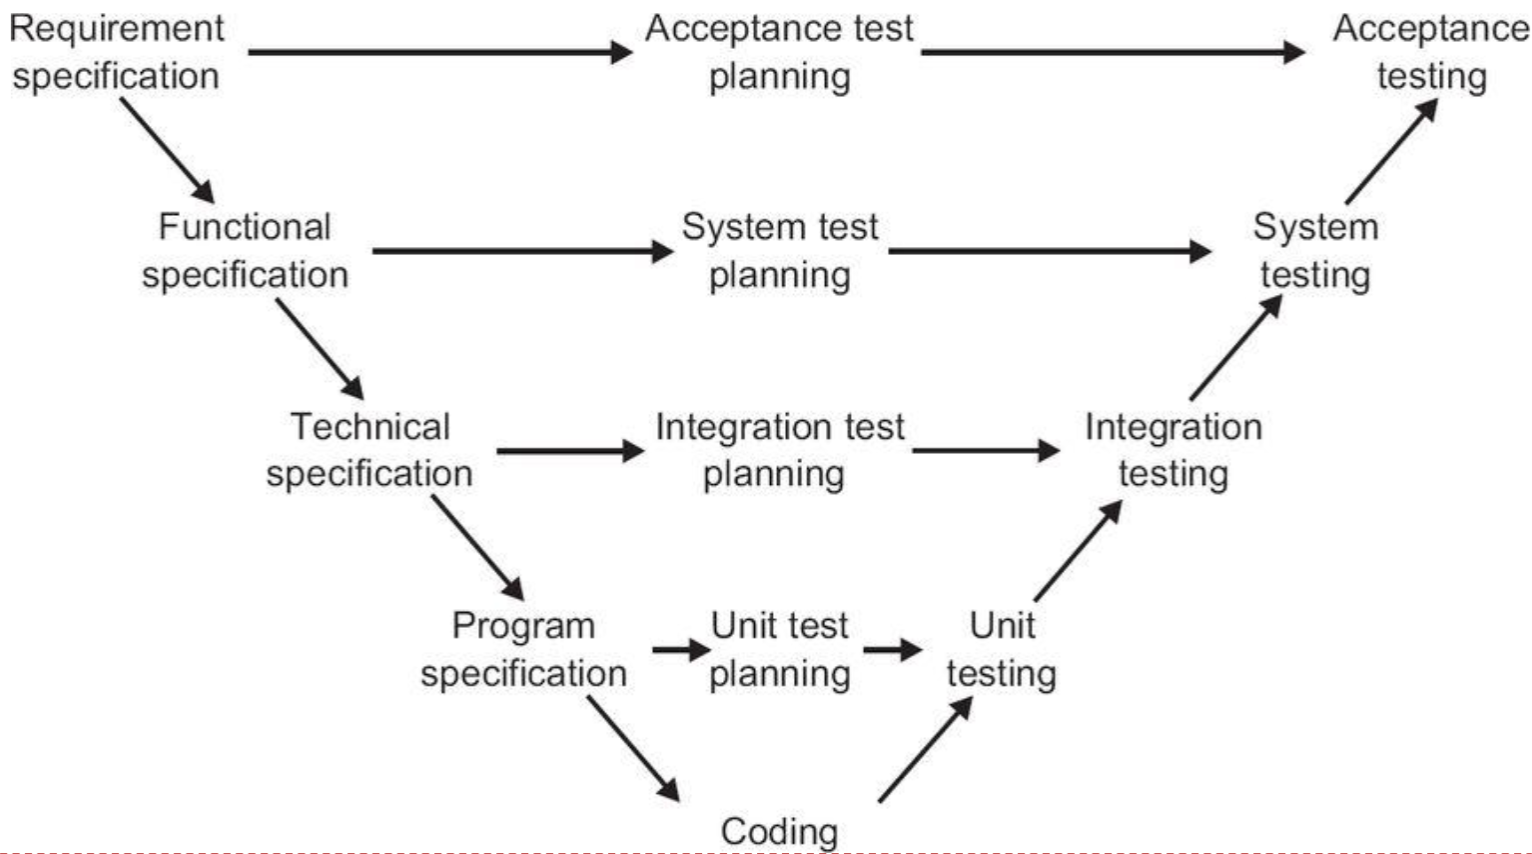
\includegraphics[width=0.7\linewidth]{Images/testing/test.png}
    \caption{Schema processo di testing.}
\end{figure}

\section{Componenti del Testing}
Si divide in:
\begin{itemize}
    \item \textbf{\textcolor{brown}{Test basis:}} tutto il materiale utilizzato per il test.
    \item \textbf{\textcolor{brown}{Test condition:}} condizioni che siano rispettate che vengono simulati, cerca di vagliare tutte le condizioni.
    \item \textbf{\textcolor{brown}{Test case:}} si simula un comportamento o una operazione basato sulle prime due tecniche.
    \item \textbf{\textcolor{brown}{Test procedure:}} sono il complesso delle attività che facciamo per portare a termine il test.
\end{itemize}

Per stabilire i test case posso usare \textbf{\textcolor{blue}{tecniche di testing}}:
\begin{itemize}
    \item Basate sull'\textbf{intuizione}: con esperienza e beta-testing, quando l'utente ha testato il prodotto senza vincoli avrò degli utenti esperti che insegnano.
    \item Basate sulle \textbf{specifiche}: con test \textbf{black-box}, senza esaminare il codice, che si basa sul comportamento del sistema con tecniche \textbf{ECP}, \textbf{BVA}.
    \item Basate sul \textbf{codice}: con test \textbf{white-box}, sfruttando la conoscenza del codice sorgente analizzando tutti i percorsi cercando la massima copertura.
    \item Basate su \textbf{test esistenti}: con \textbf{regression testing}, riutilizzando test precedentemente creati per verificare che non si siano reintrodotti i difetti.
    \item Basate sugli \textbf{errori}: tramite tentativi di indovinare basati sull'esperienza o analisi di porzioni di codice che tendenzialmente sono propense a difetti.
\end{itemize}

\section{Processo di Testing}
Diversi processi di test:
\begin{itemize}
    \item \textbf{\textcolor{brown}{Test planning:}} devo pianificare che cosa deve essere testato e quali sono gli obiettivi da raggiungere, per fare test organizzati, tracciabili, allineati.
    \item \textbf{\textcolor{brown}{Test monitoring e controllo:}}stabilire delle misure di controllo e monitoraggio per vedere se sono raggiunti gli obiettivi tramite dei criteri d'uscita.
    \item \textbf{\textcolor{brown}{Test analysis:}} esaminare le basi di test per identificare cosa c'è bisogno di testare, stabilendo una priorità di testing.
    \item \textbf{\textcolor{brown}{Test design:}} scrivere i test case per valutare come bisogna testare ciò che è emerso con l'analisi, sfruttando le condizioni di test.
    \item \textbf{\textcolor{brown}{Test implementation:}} comprendere come introdurre i parametri dentro il codice e scrivere le porzioni di codice per eseguirlo, creare l'ambiente.
    \item \textbf{\textcolor{brown}{Test execution:}} eseguire nella pratica il test appena costruito e registrare i risultati.
    \item \textbf{\textcolor{brown}{Test completion:}} terminazione della fase di testing per rilasciare una versione con un report degli errori corretti.
\end{itemize}

\section{Processo di revisione}
Si distingue la review \textbf{informale}, una discussione ad hoc da quella \textbf{formale}, tramite delle rigide procedure, risultati documentati e ruoli definiti. \\
Gli obiettivi sono trovare i difetti, comprendere il prodotto e generare delle discussioni tra i membri, scambiare la conosce nza e decidere con coscienza.

\begin{figure}[!htb]
    \centering
    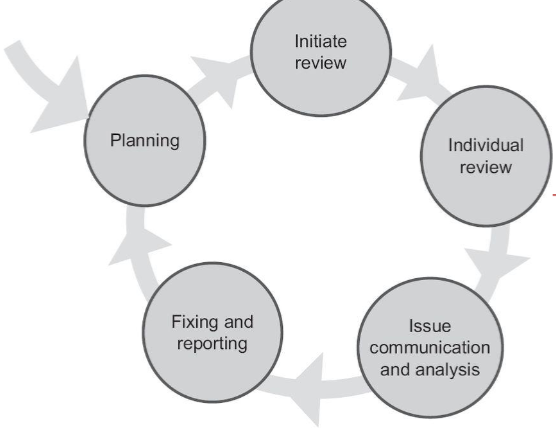
\includegraphics[width=0.5\linewidth]{Images/testing/review.png}
    \caption{Schema di review.}
\end{figure}